\scanpage{49}
\mspage{5)}
% archive sheet number: 48
Cette opération de somme est la plus triviale parmi les opérations qu'il nous faudra expliciter et transcrire (combinatoirement) dans la suite. Notons de suite, pour $(X,\widetilde{\Sigma},R)$, donné
\[
X\ \deleted{\unsure{\text{est}}}\text{connexe}
\quad\Longleftrightarrow\quad
\Gamma\mathrm{MD}(X,\widetilde{\Sigma},R)\ \text{connexe}
\]
plus précisément
\[
\pi_{0}(X)\simeq\pi_{0}(\Gamma\mathrm{MD}(X,\widetilde{\Sigma},R))
\]
% slanted
\margin{dans ce cas formule pour le genre d'une $\alpha\in\pi_{0}(X)\simeq\pi_{0}(\Gamma)$ en termes de la pondération --- plus généralement, $\unsure{g_s}$ donné par $\Gamma$. Le \uline{genre total} est $g=\sum_{s\in S}g_{s}+c(\Gamma)$, \unsure{indice de connexion|indice de connexité} du graphe $\unsure{=\mathrm{rg}}\,H_{1}(\Gamma)$ \deleted{\unsure{\mathrm{caract.}}}}

\uline{Cas particuliers}.

a) Cas de $S_{*}{\unsure{\mathscr T|\mathcal T}}_{\mathrm{top}}^{\pm}\ \deleted{\unsure{S_{*}\mathscr{T}D_{\mathrm{top}}}}$ --- ici $\Sigma=\unsure{\varnothing|\phi}$, $\widetilde{\Sigma}=\partial X$.

Cela correspond \unsure{à ce que|au cas où} les graphes MD \deleted{qui} où \inserted{toutes les arêtes sont libres, i.e.} tous les sommets sont isolés (sauf arêtes libres) \deleted{\unsure{Le}} \inserted{Ce graphe} est donc déterminé par
\diagram{
\begin{tikzcd}[ampersand replacement=\&]
A\ (\unsure{\simeq|=} \vec A\,\unsure{=|-}\,\vec A^{\sigma})\arrow[d]\arrow[r,"\unsure{r|\rho}"]\&\mathbb N\\
S\arrow[r,"\gamma"]\&\mathbb N
\end{tikzcd}
}
Le cas de $\mathscr T_{\mathrm{top}}^{\pm}$ correspond à choisir $\rho=0$, donc la situation est donnée par
\figure{
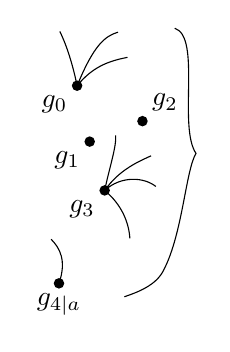
\begin{tikzpicture}[x=1cm,y=1cm]
\coordinate (a) at (.38,3); \coordinate (d) at (.73,1.67); \coordinate (e) at (.15,.49);
\draw (a) .. controls (.31,3.34) and (.22,3.57) .. (.16,3.69)
      (a) .. controls (.59,3.51) and (.73,3.63) .. (.9,3.68)
      (a) .. controls (.57,3.23) and (.76,3.31) .. (1.02,3.36);
\draw (d) .. controls (.79,1.96) and (.88,2.22) .. (.87,2.37)
      (d) .. controls (.92,1.94) and (1.17,2.04) .. (1.32,2.11)
      (d) .. controls (.94,1.86) and (1.23,1.84) .. (1.38,1.72)
      (d) .. controls (.96,1.48) and (1.04,1.24) .. (1.05,1.06);
\draw (e) .. controls (.25,.78) and (.16,.94) .. (.05,1.05);
\fill (a) circle (1.9pt) node[below left] {$g_0$};
\fill (.54,2.29) circle (1.9pt) node[below left] {$g_1$};
\fill (1.21,2.55) circle (1.9pt) node[above right] {$g_2$};
\fill (d) circle (1.9pt) node[below left] {$g_3$};
\fill (e) circle (1.9pt) node[below] {$g_{\unsure{4|a}}$};
\draw (1.62,3.73) .. controls (1.96,3.62) and (1.66,2.48) .. (1.89,2.14)
      .. controls (1.76,1.93) and (1.72,1.12) .. (1.48,.66)
      .. controls (1.39,.47) and (1.16,.38) .. (.98,.32);
\end{tikzpicture}
}
\diagram{
\begin{tikzcd}[ampersand replacement=\&]
A=\unsure{A_0|A_\ell}\arrow[d]\&\\
S\arrow[r,"\gamma"]\&\mathbb N\quad .
\end{tikzcd}
}
\deleted{type $(g,\nu)$ d'un \unsure{sommet}} Le cas d'une situation connexe ($\mathrm{card.}\,S=1$ \inserted{i.e. $S=\{s\}$}) est \deleted{\unsure{bien caractérisé par le genre}} \inserted{caractérisé} par la donnée des deux entiers $(g,\unsure{\nu|v})$ ($g=$ genre, $\nu=$ nb de trous)
\[
g=\gamma(s),\quad \unsure{\nu|\gamma}=\mathrm{card}\, A
\]
